\documentclass[12pt,a4paper]{article}

\usepackage{graphicx}
\usepackage{abstract}
\usepackage{hyperref}
\usepackage{listings}
%\usepackage{indentfirst}  % Can be finicky. Use primarily for homework.
\usepackage{amssymb}

\graphicspath{ {./images/} }
\renewcommand{\abstractname}{\large{Timestamps}}

\setlength{\parindent}{0.5in}

\title{CPSC 323 - Lecture}
\author{Chris Nutter\thanks{Dedicated to @QuesoGrande a.k.a. Jared D.}}

% --> Here we go, satellite radio, y'all get hit with a...

\begin{document}

\maketitle

\begin{abstract}
    \noindent
    \begin{center}\textbf{09/17/2020 - 07:02:20 PM}\end{center}
        Make sure to submit project by 09-29-2020 by \textbf{ALL} group members.
    
\end{abstract}

% --> First Chapter

\section{Lecture}
    \begin{figure}[!htb]
        \centering
        \fbox{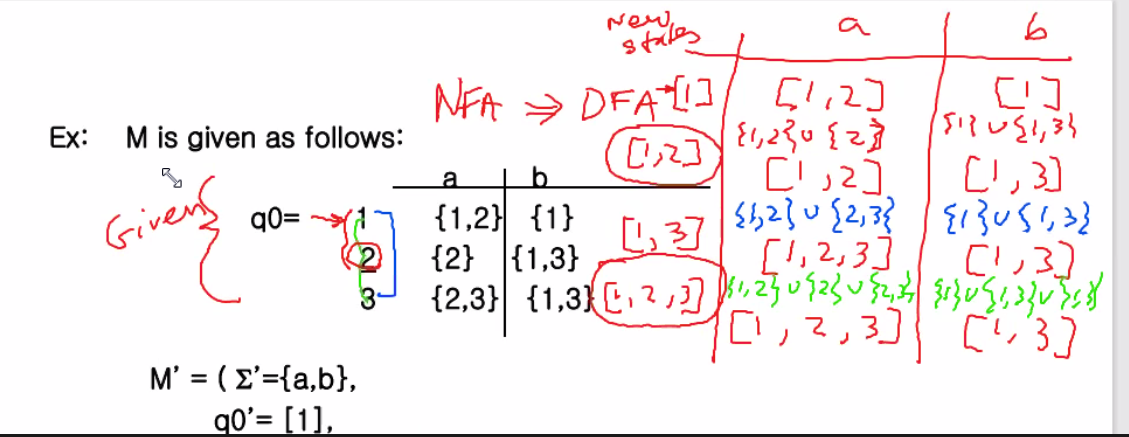
\includegraphics[width=13.5cm]{nfa-dfa.png}}
        \caption{NFA to DFA Conversion}
    \end{figure}
    \begin{figure}[!htb]
        \centering
        \fbox{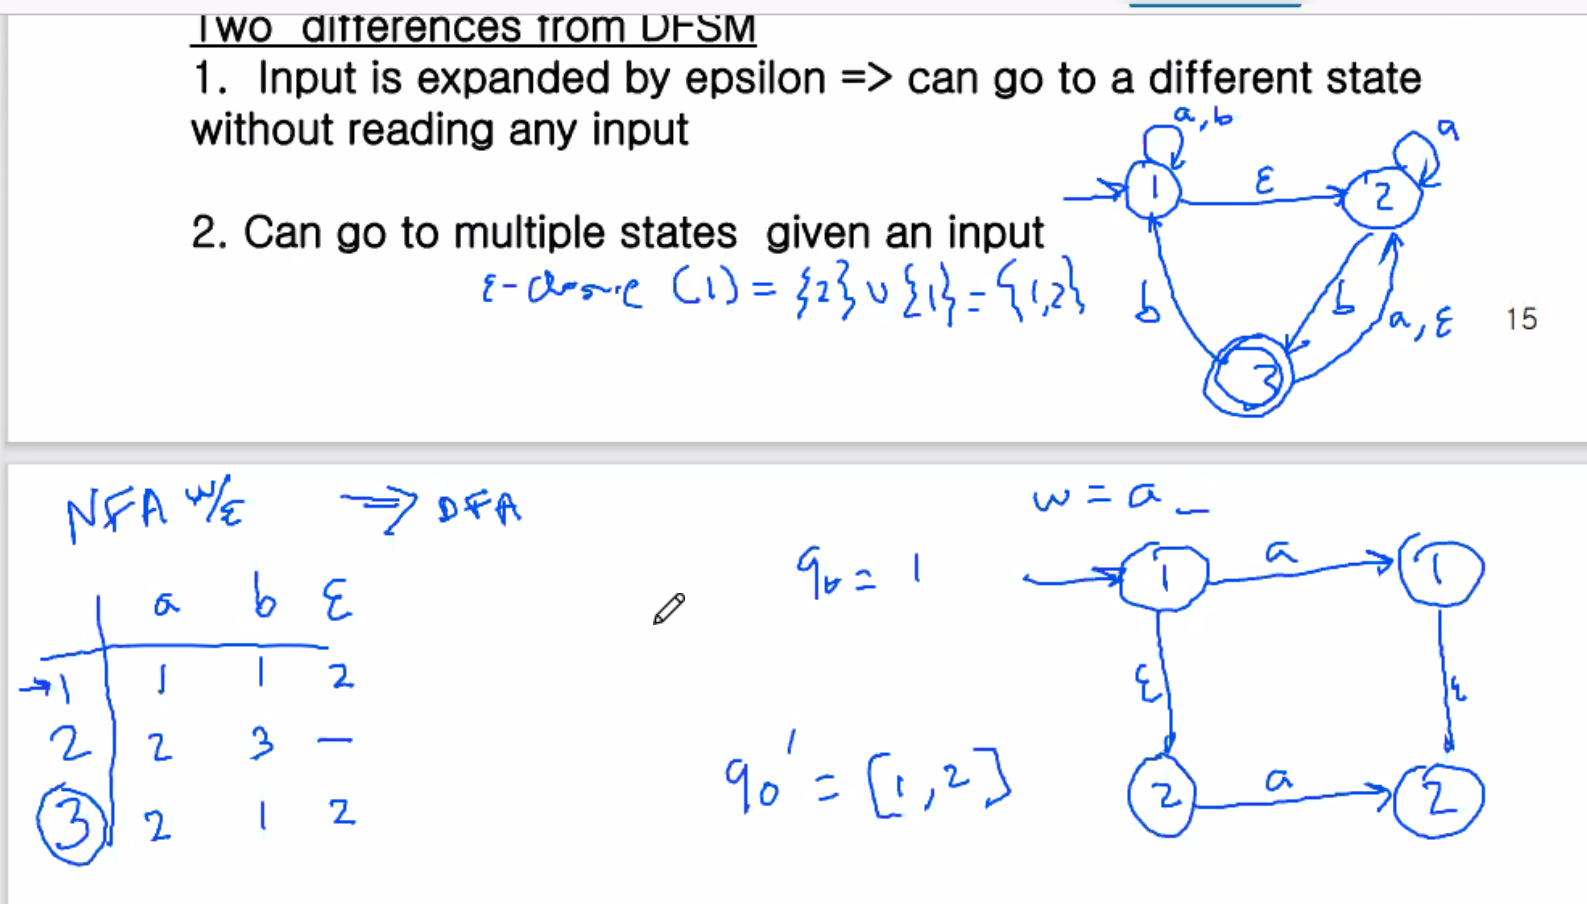
\includegraphics[width=13.5cm]{dfsm-difference.png}}
        \caption{DFSM Differences}
    \end{figure}



% --> Next Chapter

\end{document} 

% Possibly Important LaTeX Functions %
% ================================== %

%   \begin{figure}[!htb]
%       \centering
%       \fbox{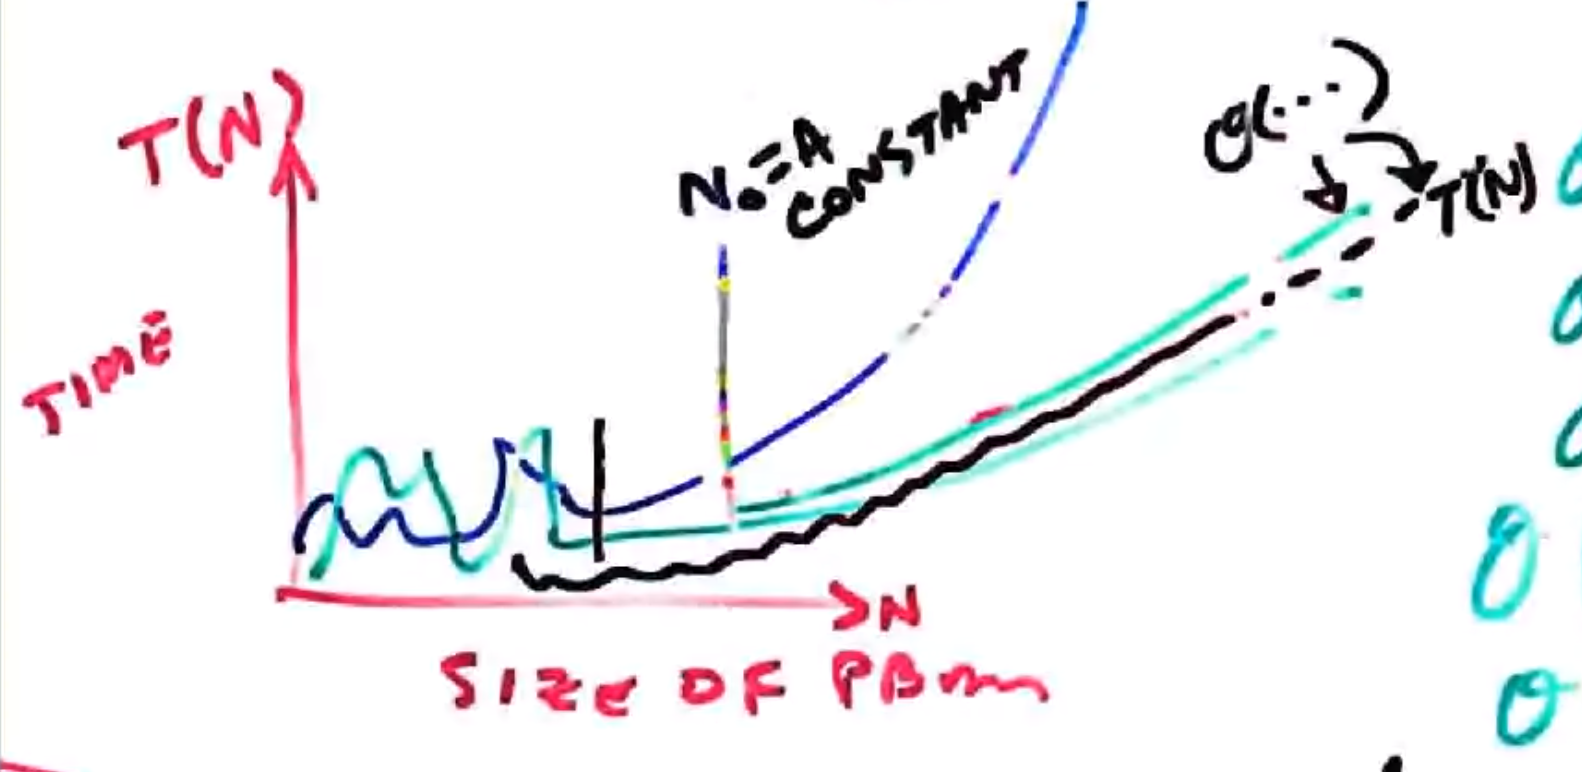
\includegraphics[width=13.8cm]{big_o.png}}
%       \caption{Big(O) Notation}
%   \end{figure}

%   \begin{lstlisting}[language=Python] 
%        print('hello world') 
%   \end{lstlisting}  

